\section{Preliminary}
We consider a conversational setting in which a user interacts with an assistant agent over time. Let \( h_t \) denote the \( t \)-th dialogue snippet, and let the cumulative interaction history be represented as a dialog set
\(
\mathcal{H} = \{h_1, h_2, \ldots, h_t\}.
\)
To support long-term personalization, the system maintains a \textbf{user memory bank} \( \mathcal{M}_t \), a textual representation that evolves dynamically as new user behaviors and preferences emerge.
Beyond dialogue content \( h_t \), we incorporate a learnable \emph{memory-update prompt} \( \mathcal{S} \) as a parameterized system component that regulates how memory is updated.
Formally, the overall memory bank-evolution process is summarized in generic form with an evolution module \( \mathcal{T} \):
\begin{equation}
\mathcal{M}_{t+1} = \mathcal{T}(\mathcal{M}_t, h_t ; \mathcal{S}, \phi),
\end{equation}
where $\phi$ denotes the parameters of LLM. The evolution operator \( \mathcal{T} \) encapsulates the mechanisms for incorporating new information, refining existing entries, and removing outdated or inconsistent content. This formulation treats user memory as a continuously adapting latent structure aligned with the user’s evolving profile.

Given a task or query input \( x \), the agent \( \mathcal{A} \) generates a personalized response conditioned on \( x \) and the current memory state \( \mathcal{M}_t \):
\(
y_t = \mathcal{A}(x, \mathcal{M}_t),
\)
indicating that \( \mathcal{M}_t \) serves as auxiliary context modulating the agent’s behavior. The central challenge in our task, therefore, lies in designing a principled mechanism  \( \mathcal{T} \) that allows \( \mathcal{M}_t \) to evolve coherently with \( \mathcal{H} \), enabling the agent to maintain stable, accurate, and temporally consistent user representations throughout long-term interaction.




\section{Methodology}
We propose a two-stage framework for learning an effective memory-evolution mechanism. Instead of hand-crafting the update rule inside the evolution operator \( \mathcal{T} \), we treat the memory update instruction as an optimizable natural-language parameter and learn it from data. In the first stage, \textbf{Memory Guideline Induction}, we learn how the agent performs memory operations by inducing a high-quality textual guideline. Subsequently, we further optimize what to store in accordance with this guideline. The two stages are shown in Figure~\ref{fig:method}.

\begin{figure*}
\centering
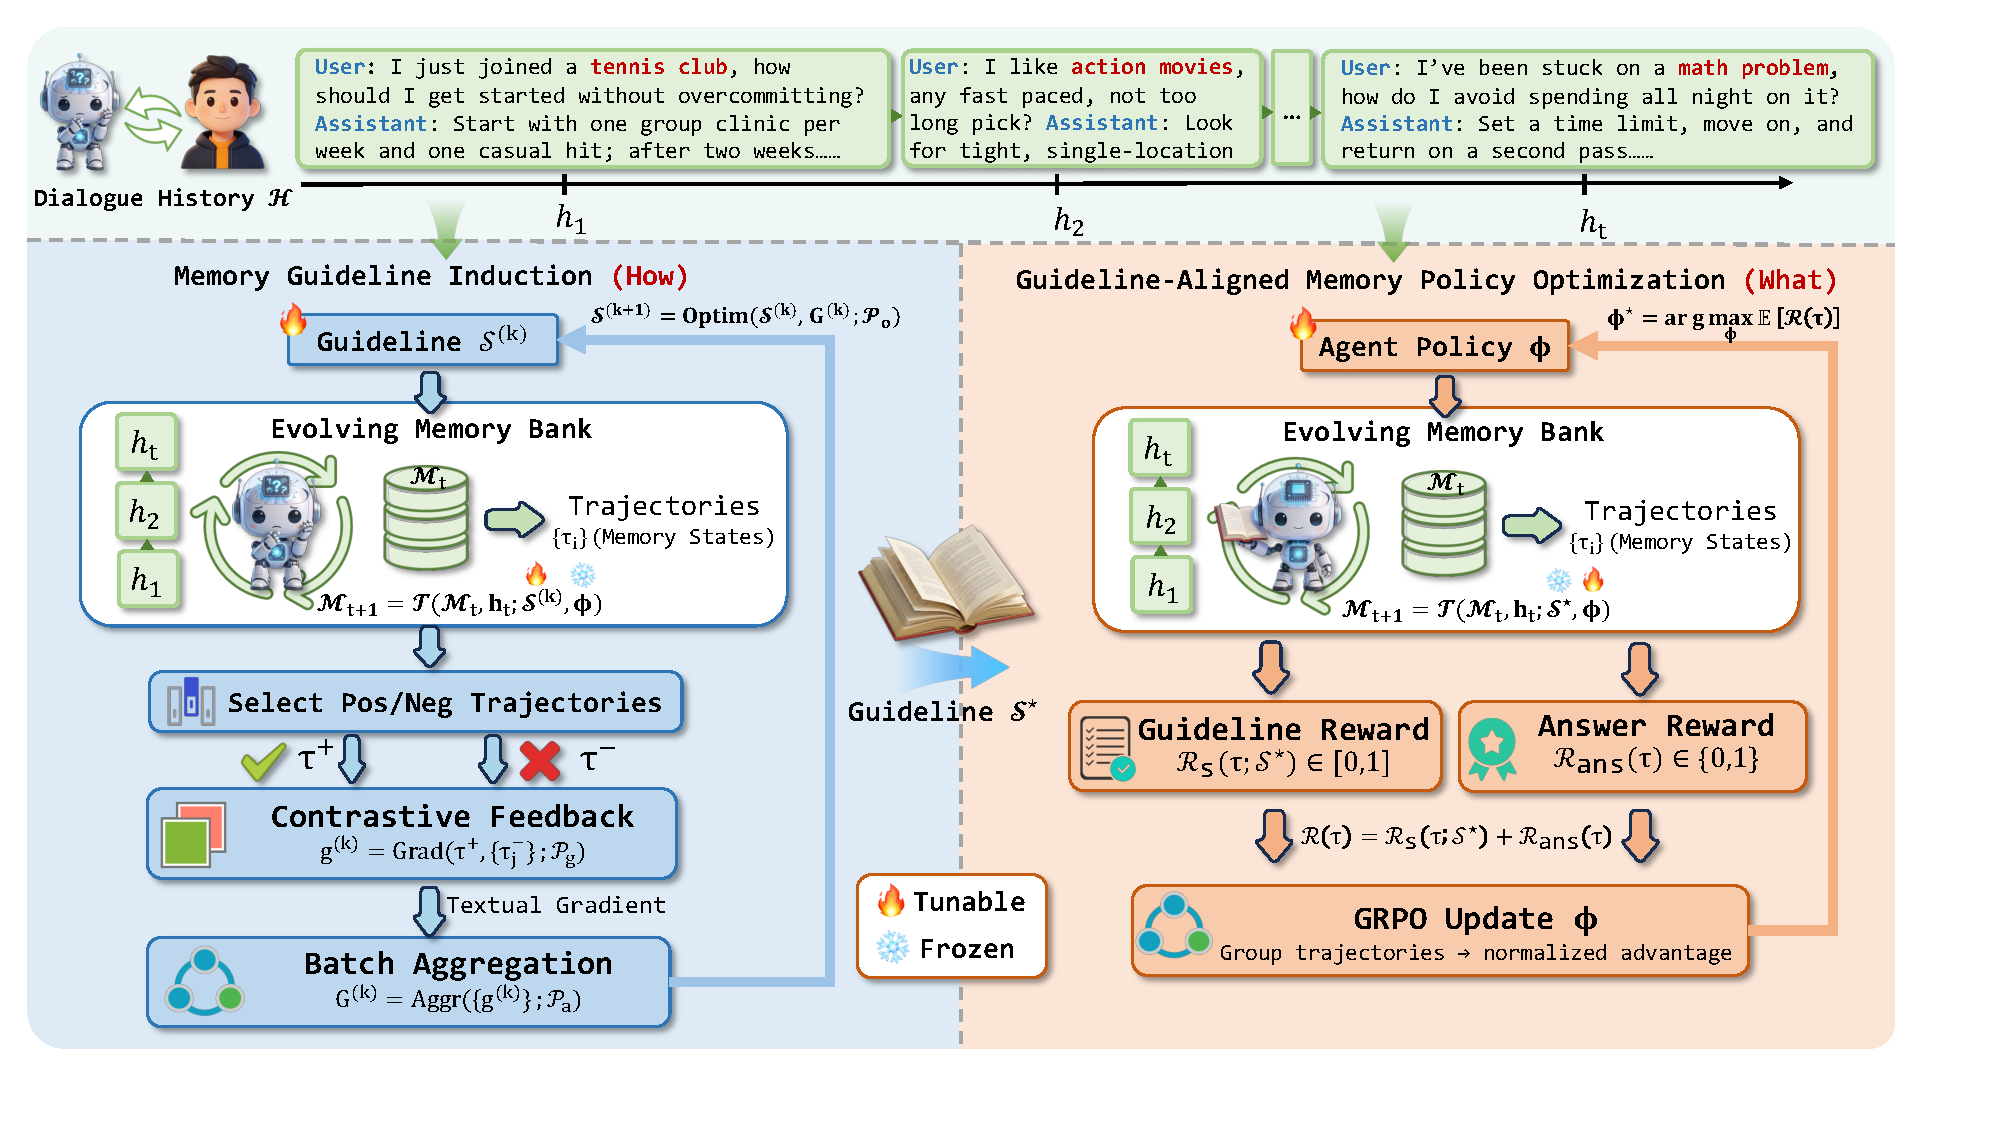
\includegraphics[width=0.99\linewidth]{img/method.pdf}
\caption{Overview of our proposed \ourmodel. It performs two-stage optimization for evolving user memory: (1) {Memory Guideline Induction} (\moduleone) iteratively refines a natural-language guideline; (2) {Guideline-Aligned Memory Policy Optimization} (\moduletwo) fixes the induced guideline to define guideline-aligned rewards and applies multi-turn GRPO to learn what information to update in evolving memory bank.}
\label{fig:method}
\end{figure*}
\subsection{Memory Guideline Induction}
\label{subsec:memory_guideline}

Existing implementations of memory-evolution methods typically rely on manually designed templates or prompts that prescribe how new dialogue segments should modify the user's memory. Such heuristic guidelines are brittle and lack the ability to adapt across domains, user styles, and annotation conventions. Inspired by schema-based human memory mechanisms, we instead treat the instruction prompt \( \mathcal{S} \) as a global natural-language parameter encoding a structured policy for memory operations, and aim to learn it from data. Consequently, the objective of the Memory Guideline Induction stage is therefore to induce an optimized guideline \( \mathcal{S}^\star \) that teaches the agent how to perform memory evolution correctly.

\paragraph{Contrastive feedback as textual gradient.}
Firstly, we use a training set where each example provides a dialogue history \(\mathcal{H}\) and a query \(x\). At optimization step \(k\), given the current guideline \(\mathcal{S}^{(k)}\), we first run the memory-evolution operator over the history and then perform multiple forward propagations of the agent to answer the query. This produces a set of trajectories \(\{\tau_i\}\), where each trajectory \(\tau_i\) contains the query \(x\), the intermediate memory states, and a candidate response \(y_i\). Using task supervision or environment feedback, we select at least one correct trajectory \(\tau^{+}\) and treat the remaining, partially plausible but suboptimal ones as contrastive negatives \(\{\tau_j^{-}\}\).
To obtain contrastive feedback, we apply a predefined feedback instruction \(\mathcal{P}_g\) that compares the correct trajectory \(\tau^{+}\) with the negative trajectories \(\{\tau_j^{-}\}\), highlighting the desired properties of \(\tau^{+}\) and the typical errors in the negatives. The resulting natural-language contrastive reflection serves as a \textbf{textual gradient}, guiding the iterative refinement of the guidelines:
\begin{equation}
g^{(k)} = \mathrm{Grad}\big(\tau^{+}, \{\tau_j^{-}\} ; \mathcal{P}_g\big).
\end{equation}
This textual gradient is then used to update \(\mathcal{S}^{(k)}\), guiding the agent toward more reliable and task-aligned trajectories.

\paragraph{Batch-level gradient aggregation.}
To obtain a stable and general update signal, we aggregate textual gradients across a mini-batch \(B\) of training examples. Each \(g^{(k)}\) provides a localized critique about how \(\mathcal{S}^{(k)}\) should change for a specific \((\mathcal{H}, x)\); the $\mathrm{Aggr}(\cdot)$ operator synthesizes these instance-level signals into a single, abstract update direction:
\begin{equation}
G^{(k)} = \mathrm{Aggr}\big(\{g^{(k)}\}_{(\mathcal{H},x)}; \mathcal{P}_a\big),
\end{equation}
where \(\mathrm{Aggr}(\cdot)\) can be instantiated as a summarization and abstraction procedure, guided by an aggregation prompt \(\mathcal{P}_a\), that identifies common failure patterns and consolidates them into a guideline-level modification proposal.


\paragraph{Optimization objective.}
% Given the merged textual gradient \(G^{(k)}\), the guideline is updated by an optimization operator that edits \(\mathcal{S}^{(k)}\) in natural language:
By applying the merged textual gradient \(G^{(k)}\), the guideline \(\mathcal{S}^{(k)}\) is refined through an optimization operator that performs natural-language editing.
\begin{equation}
\mathcal{S}^{(k+1)} = \mathrm{Optim}\big(\mathcal{S}^{(k)}, G^{(k)};\mathcal{P}_o\big).
\end{equation}
Conceptually, this iterative procedure performs gradient-like steps on an underlying contrastive objective that promotes answers aligned with the positive references and penalizes confusing them with the negatives. Let \(\mathcal{R}(\cdot)\) denote a reward function; in our implementation, it simply indicates whether the output is correct. Under this view, the induced guideline \(\mathcal{S}^\star\) can be regarded as an approximate maximizer of the expected reward:
\begin{equation} 
\mathcal{S}^{\star}
= \arg\max_{\mathcal{S}}
\mathbb{E}_{(\mathcal{H}, x)}
\Big[
\mathcal{R}\big(\tau^{+}, \{\tau_j^{-}\} ; \mathcal{S}\big)
\Big].
\end{equation}
This yields a memory guideline that encodes effective principles for guiding downstream memory evolution, which are provided in Figure \ref{prompt:template_evolve_step50}.



\subsection{Guideline-Aligned Memory Policy Optimization}

Building on the induced guideline \( \mathcal{S}^\star \), the second stage focuses on optimizing \emph{what} to store in the user memory. We fix \( \mathcal{S}^\star \) and regard the parameters \( \phi \) of the evolution operator \( \mathcal{T} \) and the agent \( \mathcal{A} \) as a unified policy over memory-augmented trajectories. For each training instance \((\mathcal{H}, x)\), rolling out the system under \( \mathcal{S}^\star \) produces a trajectory \(\tau\) that interleaves memory updates
\(
\mathcal{M}_{t+1} = \mathcal{T}(\mathcal{M}_t, h_t ; \mathcal{S}^\star, \phi)
\)
and intermediate responses
\(
y_t = \mathcal{A}(x, \mathcal{M}_t),
\)
culminating in a final answer used for evaluation.

\paragraph{Guideline-aligned rewards.}
Our first signal is a \emph{Guideline-aware} reward that explicitly enforces the guideline induced by \( \mathcal{S}^\star \). For each memory-update segment in \(\tau\), we parse the model output and prompt LLM to score whether the update strictly follows the prescribed output format (e.g., required fields, tags, and structure). These signals are aggregated into a dense guideline reward
\(
\mathcal{R}_{\text{S}}(\tau; \mathcal{S}^\star) \in [0,1],
\)
which encourages \(\mathcal{T}\) to produce guideline-aligned, well-structured memory edits rather than arbitrary free-form text. 
 Second, an answer reward \( \mathcal{R}_{\text{ans}}(\tau)  \in \{0,1\}\) measures task correctness by directly comparing the final response in \(\tau\) with the reference answer (e.g., exact or judged match), yielding a simple correctness signal used to align the memory policy with downstream performance. The overall trajectory reward combines the two components as
\(
\mathcal{R}(\tau) = (1-\lambda) * \mathcal{R}_{S}(\tau; \mathcal{S}^\star) + \lambda *  \mathcal{R}_{\text{ans}}(\tau),
\)
where \( \lambda \) balances guideline fidelity and answer accuracy.


\paragraph{Policy optimization.}
 We optimize \( \phi \) using Group Relative Policy Optimization (GRPO) over groups of trajectories on multi-conversation memory evolution. For each \((\mathcal{H},x)\), GRPO samples a group of trajectories, computes group-normalized advantages from \( \mathcal{R}(\tau) \), and applies a clipped policy-gradient update. Abstractly, the learned guideline-aligned memory policy is obtained by
\begin{equation}
\phi^\star
=
\arg\max_{\phi}
\mathbb{E}_{(\mathcal{H},x)\sim\mathcal{D},\;
\tau \sim \pi_\phi(\cdot \mid \mathcal{H},x;\mathcal{S}^\star)}
\big[
\mathcal{R}(\tau) 
\big].
\end{equation}
More details can be seen in Appendix \ref{app:grpo}. 
In this way, the second stage learns a memory-evolution policy that follows the induced guideline while selectively storing information that is most beneficial for downstream interaction quality.
